\section{Objetivos}

\begin{itemize}
    \item Diseñar y simular un \textbf{control de ratio de caudal} para los caudales \textbf{FT10} y \textbf{FT11} en \textbf{Simulink}.

    \item Obtener la función de transferencia del nivel del tanque \textbf{T-10}.

    \item Diseñar y simular un \textbf{control en cascada de nivel a caudal} para el tanque \textbf{T-10}, considerando el lazo secundario de caudal \textbf{FC10} y el lazo primario de nivel \textbf{LC10}.

    \item Evaluar la respuesta de los controladores a partir de las gráficas solicitadas y de los \textbf{parámetros de desempeño}: porcentaje de sobreimpulso, tiempo de establecimiento y error en estado estable.
\end{itemize}

\section{Trabajo prelaboratorio}



\subsection{Control de ratio de caudal}

\begin{enumerate}[label=\arabic*)]
    \item Simule un \textbf{control de ratio de caudal} para los caudales \textbf{FT10} y \textbf{FT11} en \textbf{Simulink}, de modo que el diagrama de bloques tenga una estructura similar a la mostrada en la \textbf{Figura~\ref{fig:ratio}}. Para ello, realice lo siguiente:
    \begin{enumerate}[label=\alph*.]
        \item Obtenga o utilice funciones de transferencia previas para los flujómetros \textbf{FT10} y \textbf{FT11}. Para \textbf{FT10}, considere como entrada \textbf{u} el porcentaje de apertura de válvula \textbf{FV10/EV11} y como salida \textbf{y} el caudal de agua. Para \textbf{FT11}, considere como entrada \textbf{u} el comando de frecuencia del \textbf{VFD20} o la referencia de velocidad del \textbf{G120}, y como salida \textbf{y} el caudal de agua.

        \item Utilice el bloque \textbf{LTI System} para insertar la \textbf{función de transferencia}. Sintonice el controlador \textbf{PID} de caudal \textbf{FC11}, considerando las siguientes \textbf{especificaciones de control}: porcentaje de sobreimpulso \(<10\%\), tiempo de establecimiento \(<20\) s y error en estado estable \(<1\%\). Configure la saturación de salida del controlador como \textbf{0--60 Hz} para \textbf{VFD20} o \textbf{0--100\%} para \textbf{G120}.

        \item Inserte en \textbf{Simulink} los siguientes bloques:
        \begin{itemize}
            \item \textbf{Repeating Sequence Stair}, para generar el porcentaje de apertura de la válvula \textbf{FV10/EV11} y el valor de \textbf{ratio deseado}, con un \textbf{Sample time} de \textbf{40s}. Considere que el caudal deseado máximo posible para \textbf{FT11} es \textbf{75 l/min}.
            \item \textbf{Product}, para calcular el setpoint de \textbf{FC11} a partir del producto entre el caudal de \textbf{FT10} y el ratio deseado.
            \item \textbf{Divide}, para calcular el ratio medido \textbf{FT11/FT10}.
        \end{itemize}

        \item Simule el control de ratio de caudal con \textbf{dos valores diferentes} \(0 < [v_1,v_2] < 100\) para el porcentaje de apertura de válvula \textbf{FV10/EV11} y \textbf{tres valores diferentes} \(0 < [r_1,r_2,r_3] < 2\) para el ratio deseado. Utilice un tiempo de simulación de \textbf{160 s} y un \textit{Fixed-step size} de \textbf{0.01} o menor.
    \end{enumerate}

\begin{figure}[H]
    \centering
    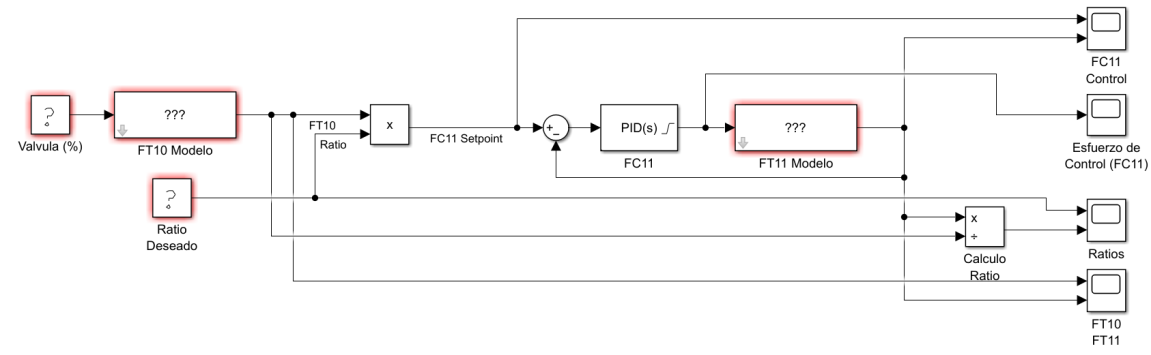
\includegraphics[width=\textwidth]{images/figure1.png}
    \caption{Diagrama de bloques en Simulink del control de ratio de caudal.}
    \label{fig:ratio}
\end{figure}

\item Presente los siguientes resultados para el \textbf{control de ratio de caudal}:
    \begin{enumerate}[label=\alph*.]
        \item Funciones de transferencia utilizadas para \textbf{FT10} y \textbf{FT11}. Muestre el \textbf{porcentaje de estimación} correspondiente.

        Las funciones de transferencia se identificaron en MATLAB mediante \texttt{procest} con estructura P1D:
        \begin{equation*}
            G_{\text{FT10}}(s) = \dfrac{1.0596}{1 + 0.376\, s}\, e^{-0.1481\, s}, \qquad \text{Fit} = 97.55\%
        \end{equation*}
        \begin{equation*}
            G_{\text{FT11}}(s) = \dfrac{0.78202}{1 + 0.48179\, s}\, e^{-0.17725\, s}, \qquad \text{Fit} = 98.29\%
        \end{equation*}

        \begin{figure}[H]
            \centering
            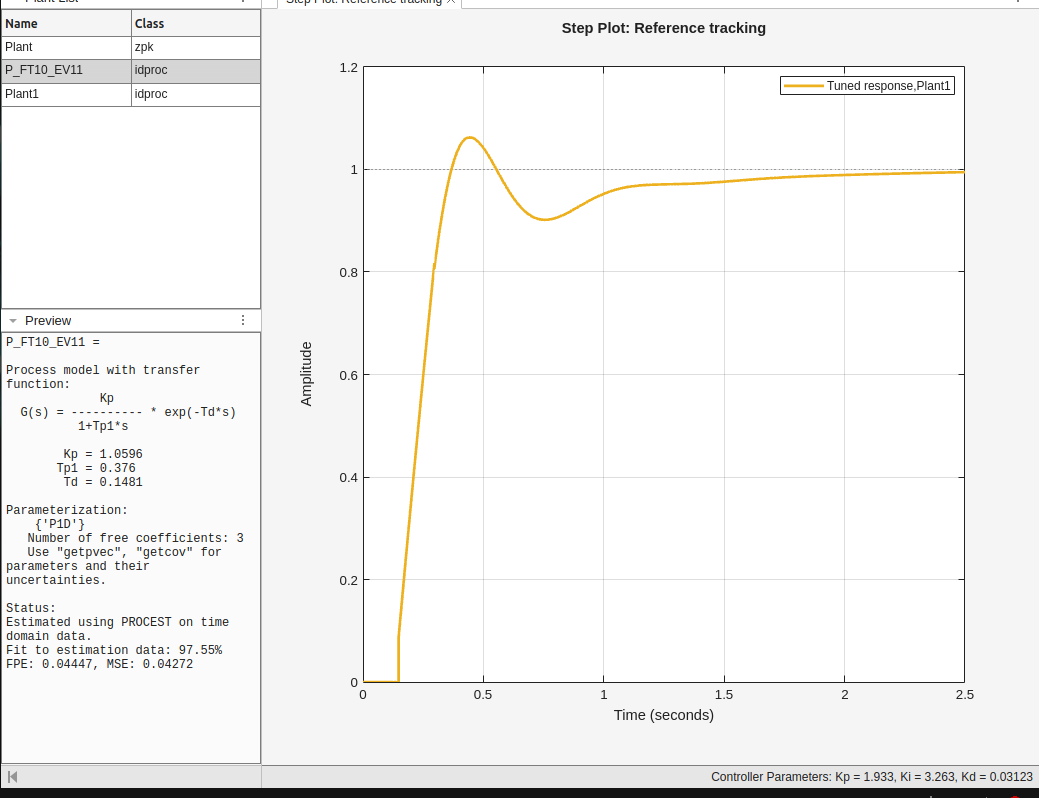
\includegraphics[width=0.85\textwidth]{images/P_FT10_EV11.png}
            \caption{Identificación de la función de transferencia FT10 (EV11 \(\rightarrow\) caudal). Fit = 97.55\%.}
            \label{fig:p_ft10}
        \end{figure}

        \begin{figure}[H]
            \centering
            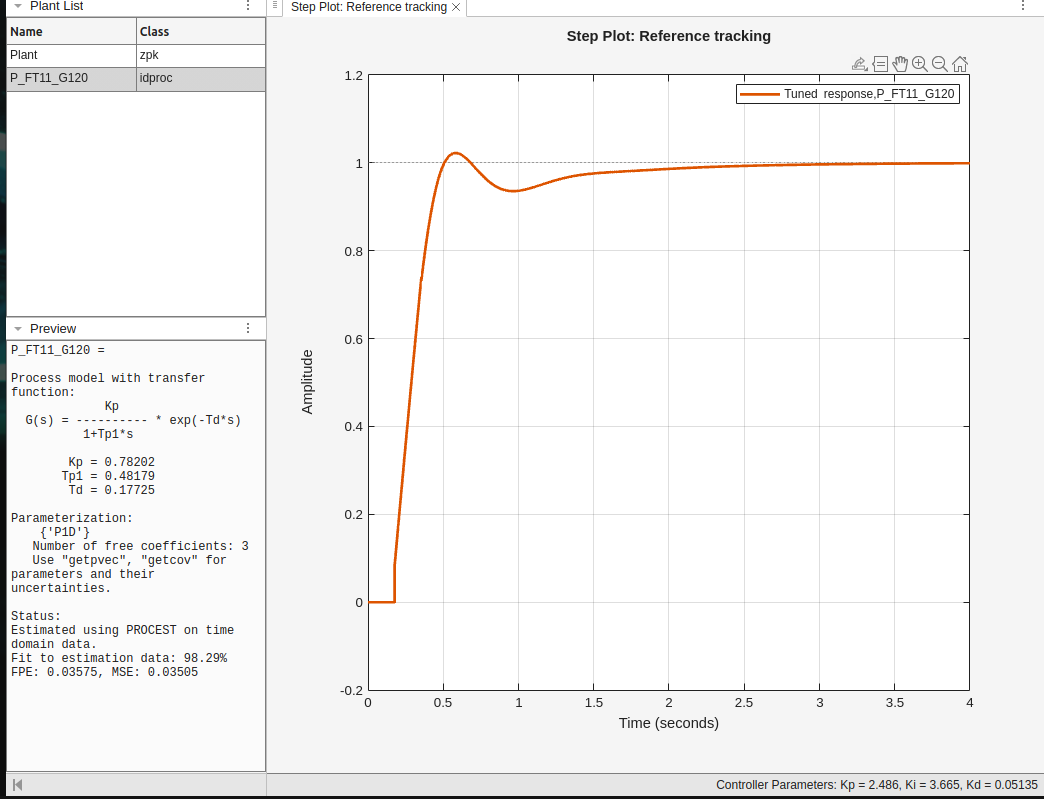
\includegraphics[width=0.85\textwidth]{images/P_FT11_G120.png}
            \caption{Identificación de la función de transferencia FT11 (G120 \(\rightarrow\) caudal). Fit = 98.29\%.}
            \label{fig:p_ft11}
        \end{figure}

        \item Ganancias del controlador \textbf{PID FC11} obtenidas.

        Las ganancias del PID FC11 obtenidas con el PID Tuner de MATLAB se presentan en la Tabla~\ref{tab:pid_fc11}.
        \begin{table}[H]
            \centering
            \begin{tabular}{|l|c|}
                \hline
                \textbf{Parámetro} & \textbf{Valor sintonizado} \\ \hline
                \(K_p\) & 2.4859 \\ \hline
                \(K_i\) & 3.6647 \\ \hline
                \(K_d\) & 0.051352 \\ \hline
                \(T_f\) & n/a \\ \hline
            \end{tabular}
            \caption{Ganancias del controlador PID FC11.}
            \label{tab:pid_fc11}
        \end{table}

        \begin{figure}[H]
            \centering
            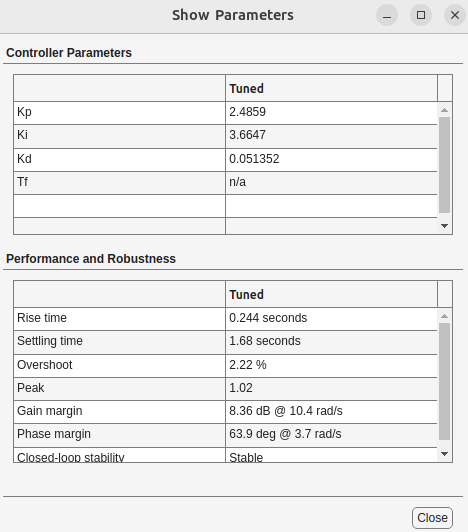
\includegraphics[width=0.65\textwidth]{images/CP_FT11_G120.png}
            \caption{Parámetros del controlador PID FC11 obtenidos en el PID Tuner de MATLAB.}
            \label{fig:cp_ft11}
        \end{figure}

        \item Imagen del \textbf{diagrama de bloques} implementado en Simulink.

        El diagrama de bloques implementado en Simulink se muestra en la Figura~\ref{fig:simulink_ratio}. Está conformado por las entradas \textbf{Valvula (\%)} y \textbf{Ratio Deseado} (Repeating Sequence Stair), las funciones de transferencia \textbf{P\_FT10\_EV11} y \textbf{P\_FT11\_G120} (LTI System), el bloque \textbf{Product} (cálculo del setpoint de FC11), el \textbf{PID FC11}, el bloque \textbf{Cálculo de Ratio} (Divide) y los \textit{Scope} de salida.
        \begin{figure}[H]
            \centering
            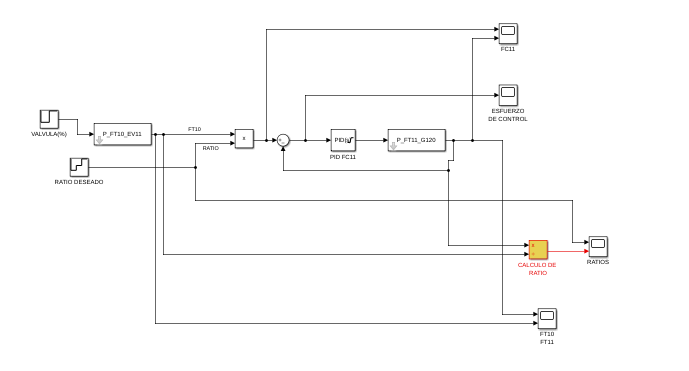
\includegraphics[width=\textwidth]{images/SIMULINK_1.png}
            \caption{Diagrama de bloques implementado en Simulink para el control de ratio de caudal.}
            \label{fig:simulink_ratio}
        \end{figure}

        \item Gráfica del control de caudal de \textbf{FT11}: setpoint de \textbf{FC11} vs. caudal medido de \textbf{FT11}.

     
        \begin{figure}[H]
            \centering
            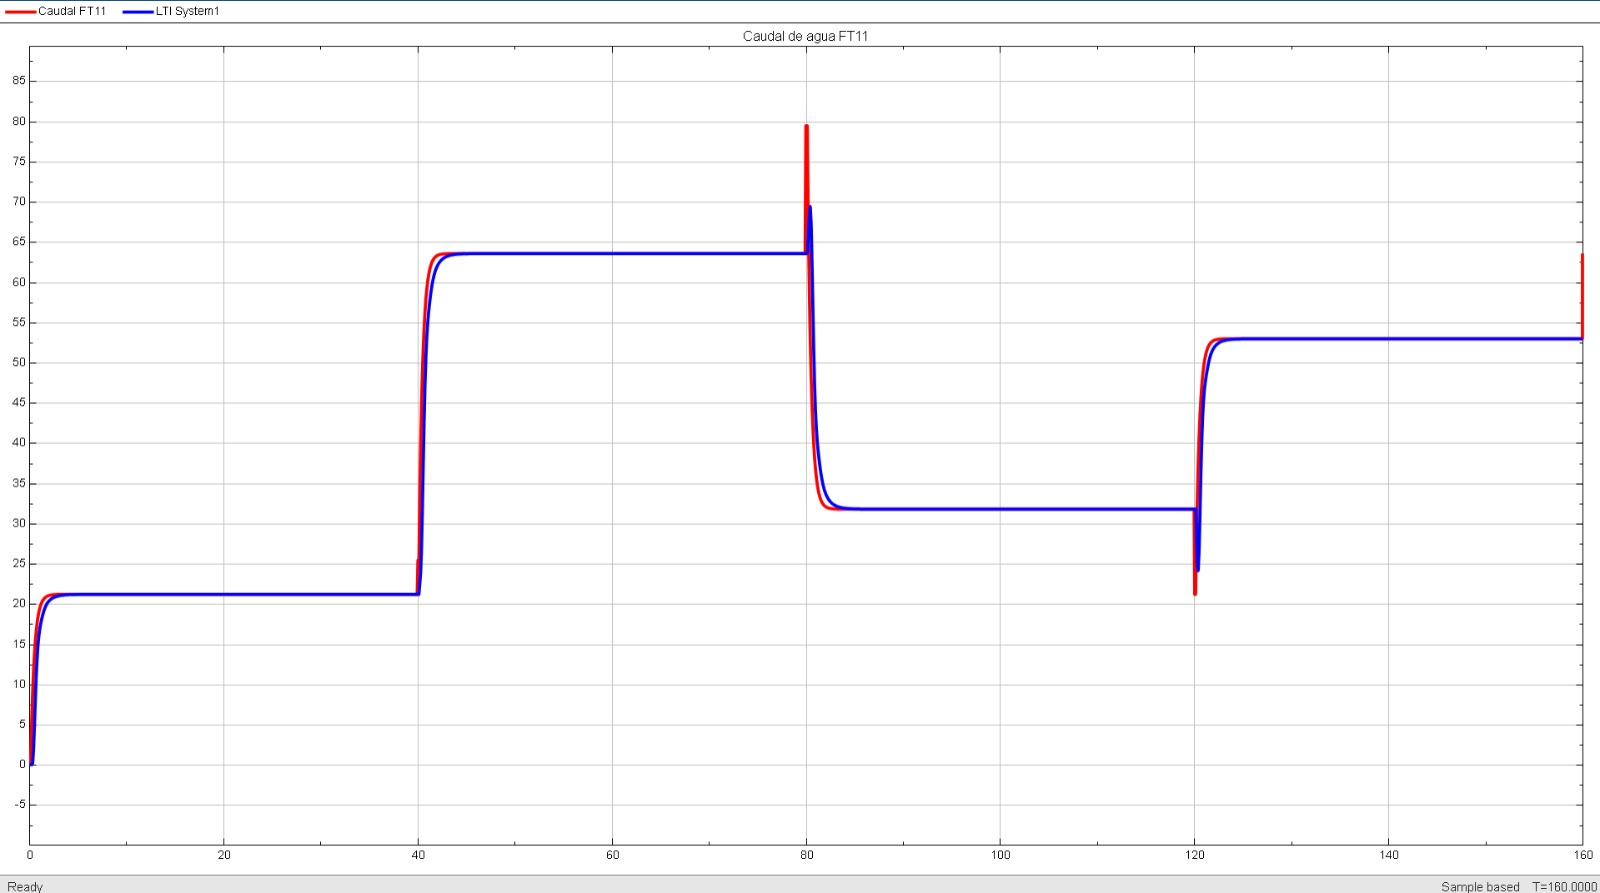
\includegraphics[width=1\textwidth]{images/FC11_CONTROL.png}
            \caption{Setpoint de FC11 vs.\ caudal medido FT11.}
            \label{fig:fc11_control}
        \end{figure}

        \item Parámetros de desempeño del control de \textbf{FT11}: porcentaje de sobreimpulso, tiempo de establecimiento y error en estado estable.

        Los parámetros de desempeño cumplen con holgura las tres especificaciones de control.
        \begin{table}[H]
            \centering
            \begin{tabular}{|l|c|c|}
                \hline
                \textbf{Parámetro} & \textbf{Valor obtenido} & \textbf{Especificación} \\ \hline
                Sobreimpulso \(M_p\) & 2.22\,\% & \(< 10\%\) \\ \hline
                Tiempo de establecimiento \(t_s\) & 1.68 s & \(< 20\) s \\ \hline
                Error en estado estable \(e_{ss}\) & \(\approx 0\,\%\) & \(< 1\%\) \\ \hline
            \end{tabular}
            \caption{Parámetros de desempeño del control de caudal FT11.}
            \label{tab:perf_fc11}
        \end{table}

        \item Gráfica del esfuerzo de control de \textbf{FC11}: frecuencia del \textbf{VFD20} o porcentaje de velocidad del \textbf{G120}.

        El esfuerzo de control (porcentaje de velocidad del G120) presenta picos transitorios en los instantes de cambio de setpoint (\(t \approx 40, 80, 120\,\)s) y se mantiene estable cercano a cero entre transiciones.
        \begin{figure}[H]
            \centering
            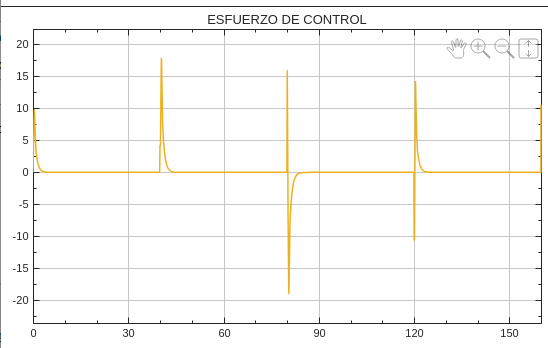
\includegraphics[width=0.9\textwidth]{images/ESFUERZO_DE_CONTROL.png}
            \caption{Esfuerzo de control de FC11: porcentaje de velocidad del G120.}
            \label{fig:esfuerzo}
        \end{figure}

        \item Gráfica comparativa del \textbf{ratio}: ratio deseado vs. ratio medido.

        El ratio medido (FT11/FT10) sigue al ratio deseado en estado estable en los cuatro segmentos. Los picos en los instantes de cambio de setpoint se deben a la división por valores transitorios pequeños de FT10.
        \begin{figure}[H]
            \centering
            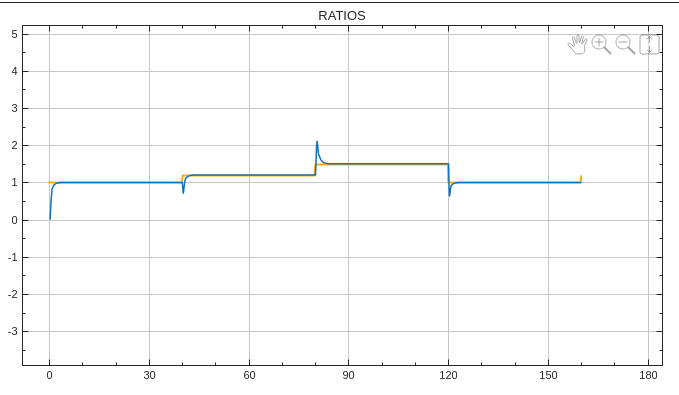
\includegraphics[width=0.9\textwidth]{images/RATIOS.png}
            \caption{Ratio deseado vs.\ ratio medido FT11/FT10.}
            \label{fig:ratios}
        \end{figure}

        \item Gráfica comparativa de caudales: \textbf{FT10} vs. \textbf{FT11}.

        Las amplitudes relativas entre FT10 (azul) y FT11 (amarillo) en cada segmento corresponden a los ratios programados (\(r_1 = 1.0\), \(r_2 = 1.2\), \(r_3 = 0.6\), retorno a \(r = 1.0\)).
        \begin{figure}[H]
            \centering
            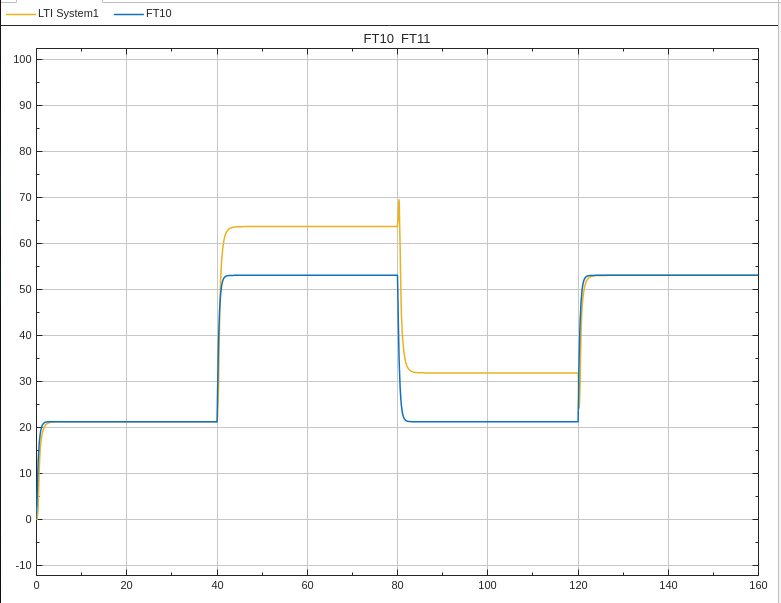
\includegraphics[width=0.9\textwidth]{images/FT10_FT11.png}
            \caption{Comparación de caudales FT10 (azul) vs.\ FT11 (amarillo).}
            \label{fig:caudales}
        \end{figure}
    \end{enumerate}
\end{enumerate}



\subsection{Control en cascada de nivel a caudal}

\begin{enumerate}[label=\arabic*)]
    \item Simule un \textbf{control en cascada de nivel a caudal} para el nivel de agua del tanque \textbf{T-10} en \textbf{Simulink}, de modo que el diagrama de bloques tenga una estructura similar a la mostrada en la \textbf{Figura~\ref{fig:cascade}}. Para ello, realice lo siguiente:
    \begin{enumerate}[label=\alph*.]
        \item Obtenga o utilice una función de transferencia previa para el flujómetro \textbf{FT10}. Considere como entrada \textbf{u} el porcentaje de apertura de válvula \textbf{FV10/EV11} y como salida \textbf{y} el caudal de agua.

        \item Obtenga una función de transferencia para el medidor de nivel. Utilice \textbf{PT11/PT10} como señal de nivel, considere como entrada \textbf{u} el caudal de agua de entrada \textbf{FT10} y como salida \textbf{y} el porcentaje de nivel de agua del tanque. Muestre el \textbf{porcentaje de estimación} de la función identificada.

        \item Inserte y sintonice el controlador secundario \textbf{PID} de caudal \textbf{FC10}, considerando las siguientes \textbf{especificaciones de control}: porcentaje de sobreimpulso \(<10\%\), tiempo de establecimiento \(<20\) s y error en estado estable \(<1\%\). Configure la saturación de salida del controlador como \textbf{0--100\%} para \textbf{FV10} o \textbf{EV11}.

        \item Inserte controlador primario \textbf{PID} de nivel \textbf{LC10} de manera externa al controlador secundario, y sintonice. Considere las siguientes \textbf{especificaciones de control}: porcentaje de sobreimpulso \(<5\%\), tiempo de establecimiento \(<200\) s y error en estado estable \(<5\%\). Configure la saturación de salida del controlador como \textbf{0--17 l/min} para \textbf{Rockwell} o \textbf{0--35 l/min} para \textbf{Siemens}.

        \item Simule el control en cascada de nivel a caudal con un \textbf{setpoint de nivel de 50\%}. Utilice un tiempo de simulación de \textbf{300 s} y un \textit{Fixed-step size} de \textbf{0.01} o menor.
    \end{enumerate}

\begin{figure}[H]
    \centering
    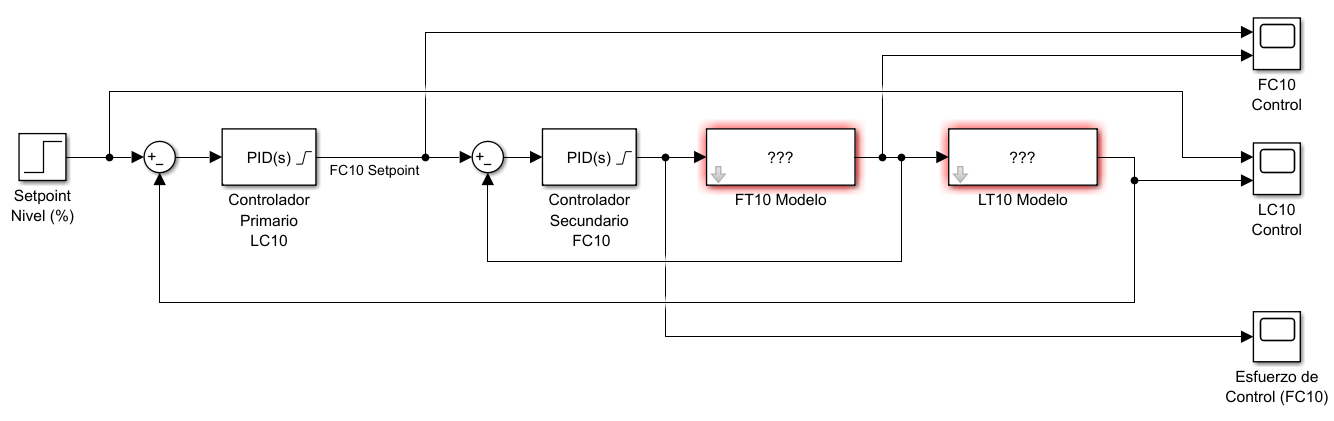
\includegraphics[width=\textwidth]{images/figure2.png}
    \caption{Diagrama de bloques en Simulink del control en cascada de nivel a caudal.}
    \label{fig:cascade}
\end{figure}



\subsection{Control en cascada de nivel a caudal}
\begin{enumerate}[label=\arabic*)]
    \item Simule un \textbf{control en cascada de nivel a caudal} para el nivel de agua del tanque \textbf{T-10} en \textbf{Simulink}, de modo que el diagrama de bloques tenga una estructura similar a la mostrada en la \textbf{Figura~\ref{fig:cascade}}. Para ello, realice lo siguiente:
    \begin{enumerate}[label=\alph*.]
        \item Obtenga o utilice una función de transferencia previa para el flujómetro \textbf{FT10}. Considere como entrada \textbf{u} el porcentaje de apertura de válvula \textbf{FV10/EV11} y como salida \textbf{y} el caudal de agua.

        Se utilizó el modelo de FT10 identificado previamente:
        \begin{equation*}
            G_{\text{FT10}}(s) = \dfrac{1.0596}{1 + 0.376\, s}\, e^{-0.1481\, s}, \qquad \text{Fit} = 97.55\%
        \end{equation*}

        \item Obtenga una función de transferencia para el medidor de nivel. Utilice \textbf{PT11/PT10} como señal de nivel, considere como entrada \textbf{u} el caudal de agua de entrada \textbf{FT10} y como salida \textbf{y} el porcentaje de nivel de agua del tanque. Muestre el \textbf{porcentaje de estimación} de la función identificada.

        Se identificó el modelo de nivel \textbf{PT10} en MATLAB con \texttt{procest} usando estructura P1 (primer orden sin retardo):
        \begin{equation*}
            G_{\text{PT10}}(s) = \dfrac{5.7577}{1 + 11.83\, s}, \qquad \text{Fit} = 82.71\%
        \end{equation*}

        \item Inserte y sintonice el controlador secundario \textbf{PID} de caudal \textbf{FC10}, considerando las siguientes \textbf{especificaciones de control}: porcentaje de sobreimpulso \(<10\%\), tiempo de establecimiento \(<20\) s y error en estado estable \(<1\%\). Configure la saturación de salida del controlador como \textbf{0--100\%} para \textbf{FV10} o \textbf{EV11}.

        El controlador FC10 (lazo interno, caudal) se sintonizó con el PID Tuner de MATLAB sobre el modelo \(G_{\text{FT10}}(s)\). La saturación de salida se configuró en \textbf{0--100\,\%} para EV11.

        \item Inserte controlador primario \textbf{PID} de nivel \textbf{LC10} de manera externa al controlador secundario, y sintonice. Considere las siguientes \textbf{especificaciones de control}: porcentaje de sobreimpulso \(<5\%\), tiempo de establecimiento \(<200\) s y error en estado estable \(<5\%\). Configure la saturación de salida del controlador como \textbf{0--17 l/min} para \textbf{Rockwell} o \textbf{0--35 l/min} para \textbf{Siemens}.

        El controlador primario LC10 (lazo externo, nivel) se sintonizó con el PID Tuner sobre el modelo \(G_{\text{PT10}}(s)\). La saturación de salida se configuró en \textbf{0--35 l/min} para Siemens.

        \item Simule el control en cascada de nivel a caudal con un \textbf{setpoint de nivel de 50\%}. Utilice un tiempo de simulación de \textbf{300 s} y un \textit{Fixed-step size} de \textbf{0.01} o menor.

        Setpoint de nivel = \textbf{50\,\%}, tiempo de simulación = \textbf{300 s}, \textit{Fixed-step size} = \textbf{0.01 s}, solver \texttt{ode4 (Runge-Kutta)}.
    \end{enumerate}

\begin{figure}[H]
    \centering
    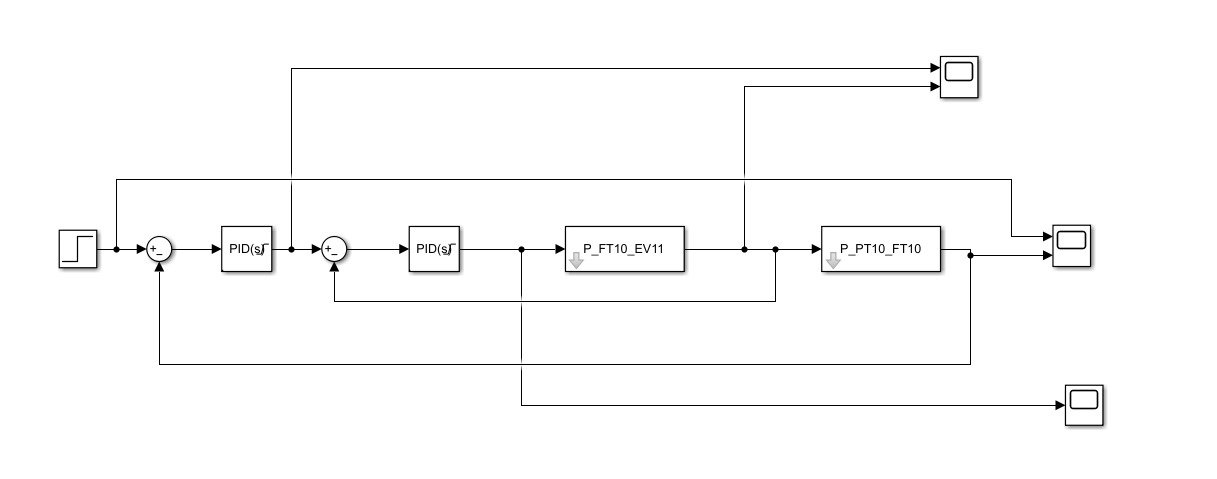
\includegraphics[width=\textwidth]{images/SIMULINK_CASCADA.png}
    \caption{Diagrama de bloques en Simulink del control en cascada de nivel a caudal.}
    \label{fig:cascade}
\end{figure}
    \item Presente los siguientes resultados para el \textbf{control en cascada de nivel a caudal}:
    \begin{enumerate}[label=\alph*.]
        \item Funciones de transferencia utilizadas para \textbf{FT10} y para el nivel del tanque \textbf{T-10}, incluyendo el porcentaje de estimación del modelo de nivel.

        Las funciones de transferencia utilizadas, identificadas con \texttt{procest} en MATLAB, son:
        \begin{equation*}
            G_{\text{FT10}}(s) = \dfrac{1.0596}{1 + 0.376\, s}\, e^{-0.1481\, s}, \qquad \text{Fit} = 97.55\%
        \end{equation*}
        \begin{equation*}
            G_{\text{PT10}}(s) = \dfrac{5.7577}{1 + 11.83\, s}, \qquad \text{Fit} = 82.71\%
        \end{equation*}

        \begin{figure}[H]
            \centering
            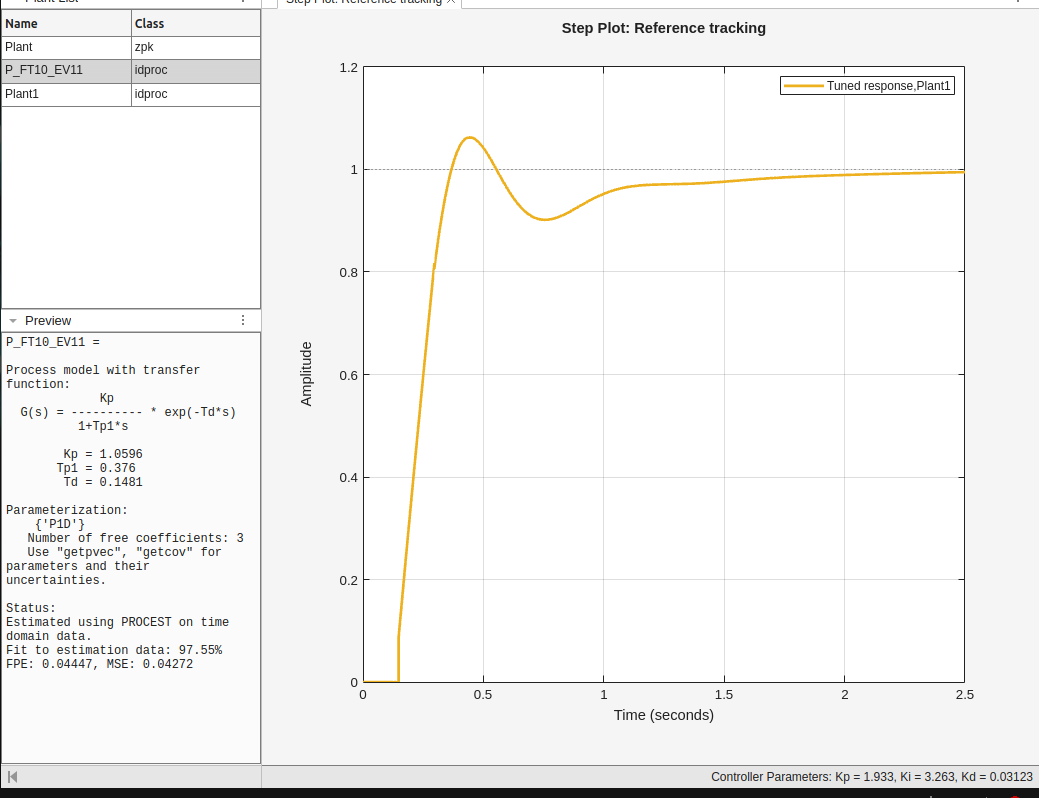
\includegraphics[width=0.7\textwidth]{images/P_FT10_EV11.png}
            \caption{Modelo P1D identificado para FT10 (EV11 \(\rightarrow\) caudal). \(K_p = 1.0596\), \(T_{p1} = 0.376\), \(T_d = 0.1481\). Fit = 97.55\%.}
            \label{fig:p_ft10_casc}
        \end{figure}

        \begin{figure}[H]
            \centering
            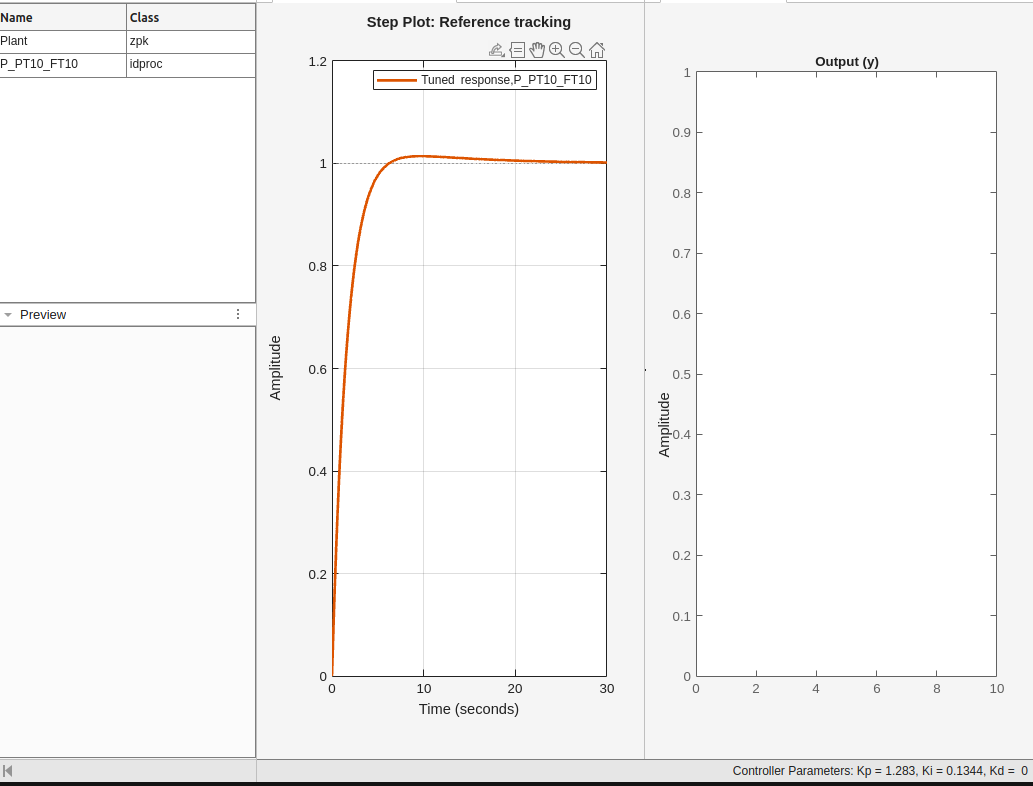
\includegraphics[width=0.7\textwidth]{images/P_PT10_FT10.png}
            \caption{Modelo P1 identificado para el nivel PT10 (FT10 \(\rightarrow\) \% nivel del tanque T-10). \(K_p = 5.7577\), \(T_{p1} = 11.83\). Fit = 82.71\%.}
            \label{fig:p_pt10}
        \end{figure}

        \item Ganancias de los controladores \textbf{PID FC10} y \textbf{LC10} obtenidas.

        Las ganancias de ambos controladores, obtenidas con el PID Tuner de MATLAB, se presentan en la Tabla~\ref{tab:pid_cascade}.
        \begin{table}[H]
            \centering
            \begin{tabular}{|l|c|c|}
                \hline
                \textbf{Parámetro} & \textbf{PID FC10 (secundario)} & \textbf{PID LC10 (primario)} \\ \hline
                \(K_p\) & 1.9328 & 1.2834 \\ \hline
                \(K_i\) & 3.2631 & 0.13437 \\ \hline
                \(K_d\) & 0.031227 & 0 \\ \hline
                \(T_f\) & n/a & n/a \\ \hline
            \end{tabular}
            \caption{Ganancias de los controladores PID FC10 y LC10.}
            \label{tab:pid_cascade}
        \end{table}

        \begin{figure}[H]
            \centering
            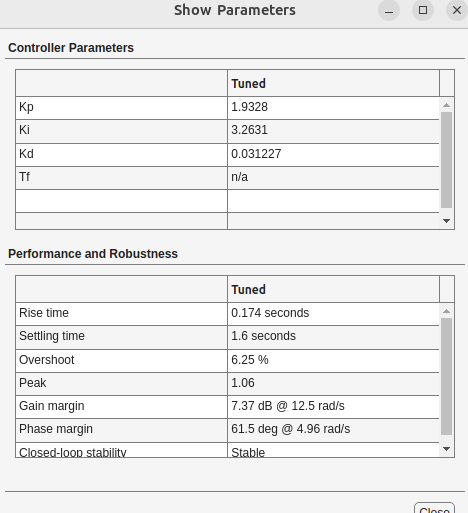
\includegraphics[width=0.6\textwidth]{images/CP_FT10_EV11.png}
            \caption{Parámetros del controlador PID FC10 (secundario, caudal) en el PID Tuner.}
            \label{fig:cp_fc10}
        \end{figure}

        \begin{figure}[H]
            \centering
            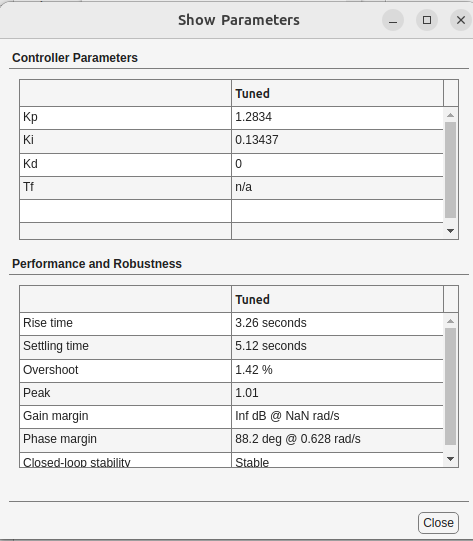
\includegraphics[width=0.6\textwidth]{images/CP_PT10_FT10.png}
            \caption{Parámetros del controlador PID LC10 (primario, nivel) en el PID Tuner.}
            \label{fig:cp_lc10}
        \end{figure}

        \item Imagen del \textbf{diagrama de bloques} implementado en Simulink.

        El diagrama implementado se muestra en la Figura~\ref{fig:simulink_cascade}. Está conformado por: el bloque \textbf{Step} (setpoint de nivel 50\,\%), el sumador del lazo externo, el \textbf{PID LC10} (primario), el sumador del lazo interno, el \textbf{PID FC10} (secundario), las funciones de transferencia \textbf{P\_FT10\_EV11} (caudal) y \textbf{P\_PT10\_FT10} (nivel), y los tres \textit{Scope} de salida (caudal FC10, nivel LC10 y esfuerzo de control).
        \begin{figure}[H]
            \centering
            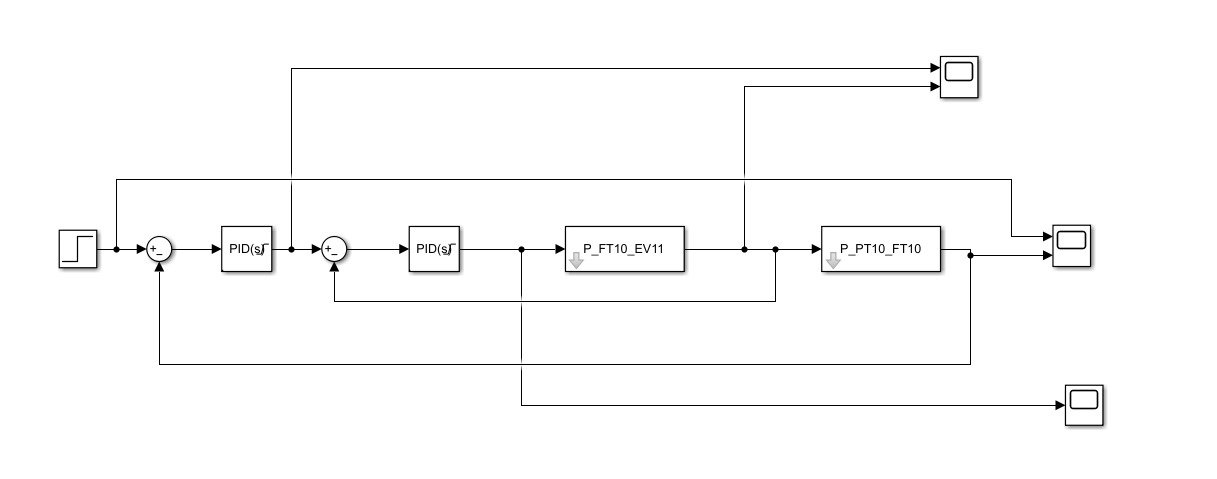
\includegraphics[width=\textwidth]{images/SIMULINK_CASCADA.png}
            \caption{Diagrama de bloques de la cascada nivel-caudal implementado en Simulink.}
            \label{fig:simulink_cascade}
        \end{figure}

        \item Gráfica del control de caudal \textbf{FC10}: setpoint de caudal vs. caudal medido de \textbf{FT10}.

        Durante los primeros 80 s el setpoint generado por LC10 alterna entre la saturación superior (35 L/min) y 0 L/min debido al \textit{wind-up} producido por el gran error inicial de nivel. A partir de \(t \approx 90\,\)s el setpoint y el caudal medido convergen y se estabilizan en aproximadamente \textbf{8.7 L/min}, valor de régimen permanente del sistema en cascada.
        \begin{figure}[H]
            \centering
            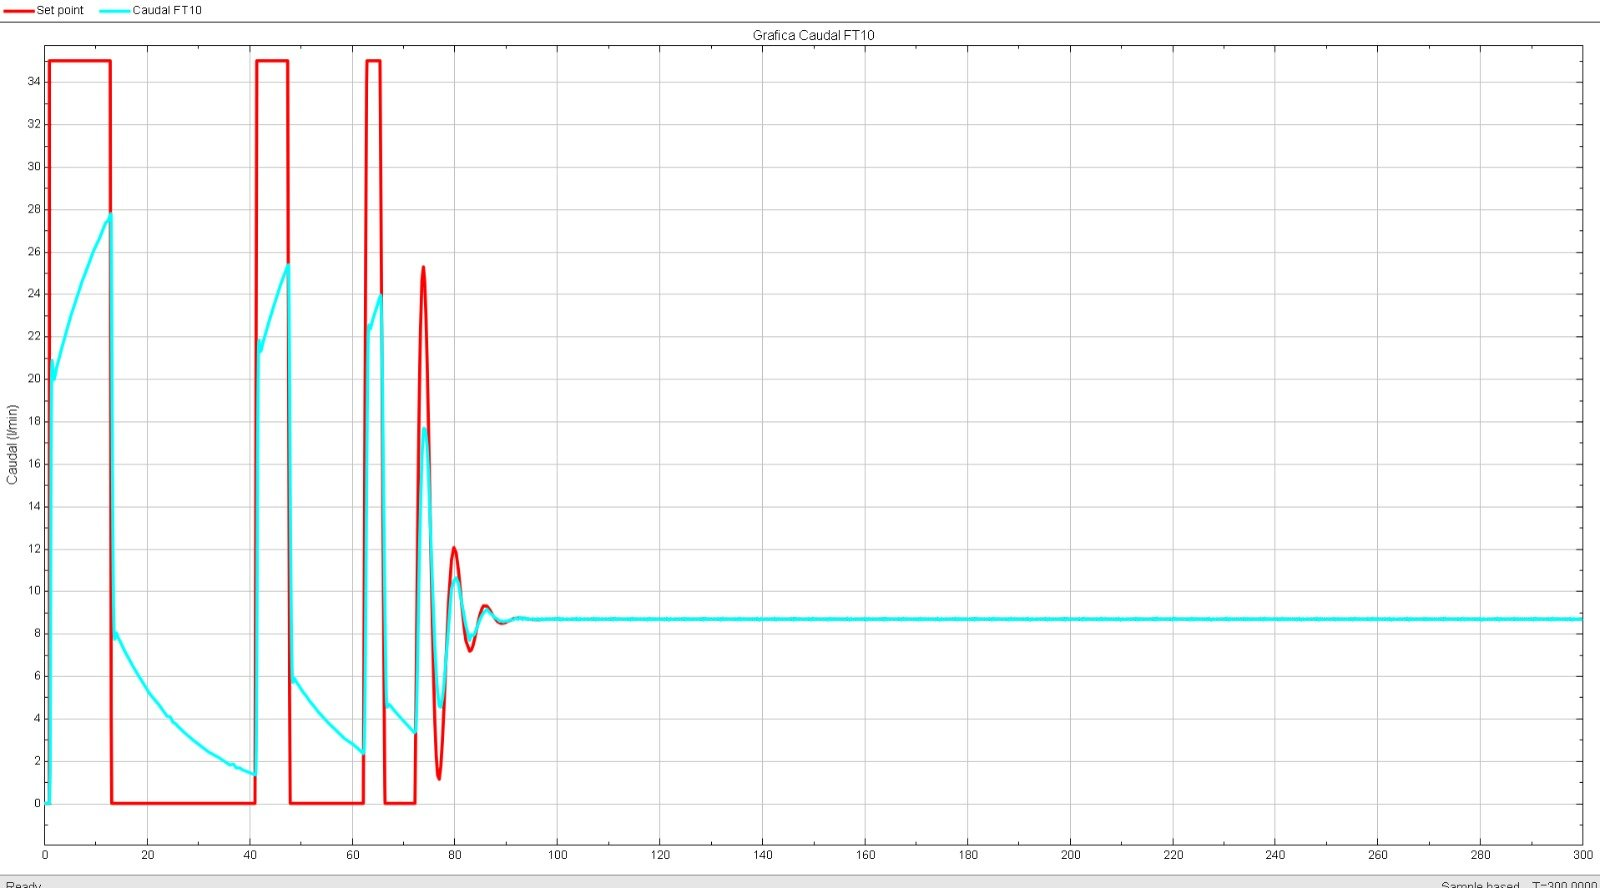
\includegraphics[width=0.95\textwidth]{images/FC10_CONTROL.png}
            \caption{Setpoint de caudal (rojo) vs.\ caudal medido FT10 (cyan).}
            \label{fig:fc10_control}
        \end{figure}

        \item Gráfica del control de nivel \textbf{LC10}: setpoint de nivel vs. nivel medido del tanque \textbf{T-10}.

        El nivel medido responde al escalón de 50\,\% con oscilaciones amortiguadas: pico inicial de \(\approx 91\,\%\) (\(t \approx 13\,\)s), seguido de oscilaciones decrecientes (69\,\%, 58\,\%, 53\,\%) hasta estabilizarse en el setpoint de \textbf{50\,\%} alrededor de \(t \approx 90\,\)s, con error en estado estable despreciable.
        \begin{figure}[H]
            \centering
            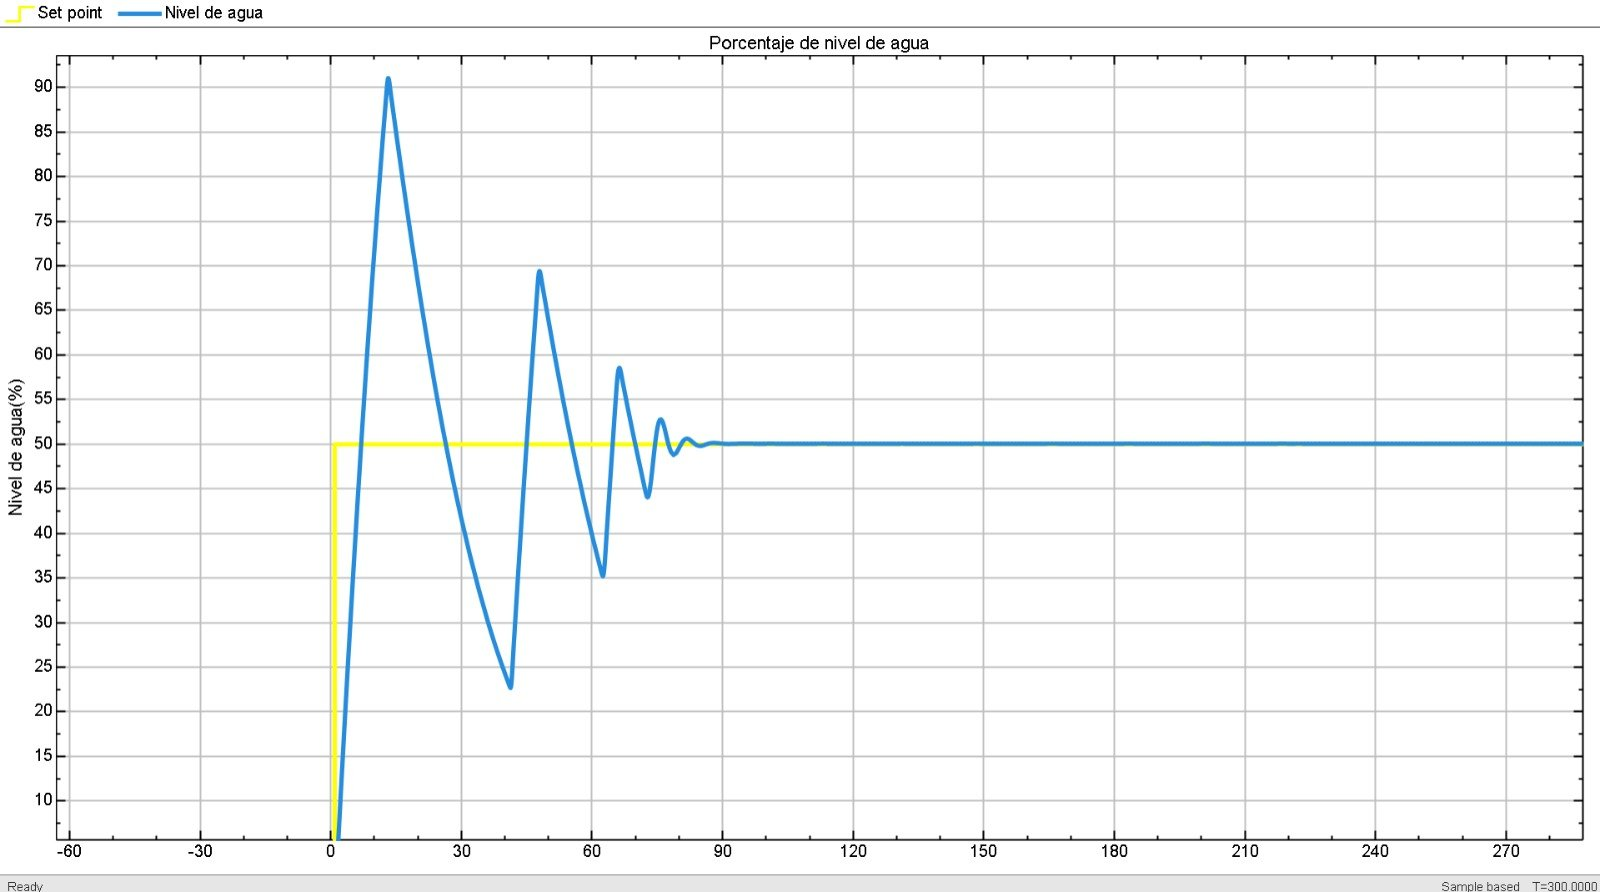
\includegraphics[width=0.95\textwidth]{images/LC10_NIVEL.png}
            \caption{Setpoint de nivel 50\,\% (amarillo) vs.\ nivel medido del tanque T-10 (azul).}
            \label{fig:lc10_nivel}
        \end{figure}

        \item Gráfica del esfuerzo de control de \textbf{FC10}: porcentaje de apertura de \textbf{FV10/EV11}.

        La apertura de EV11 presenta picos transitorios durante los primeros 80 s (máximos de 27\,\%, 35\,\% y 28\,\% en \(t \approx 13, 41, 63\,\)s), correspondientes a las oscilaciones del nivel, y se estabiliza en aproximadamente \textbf{8.2\,\%} en régimen permanente. La señal nunca alcanza la saturación de 100\,\%, lo que indica que el actuador opera dentro de su rango lineal.
        \begin{figure}[H]
            \centering
            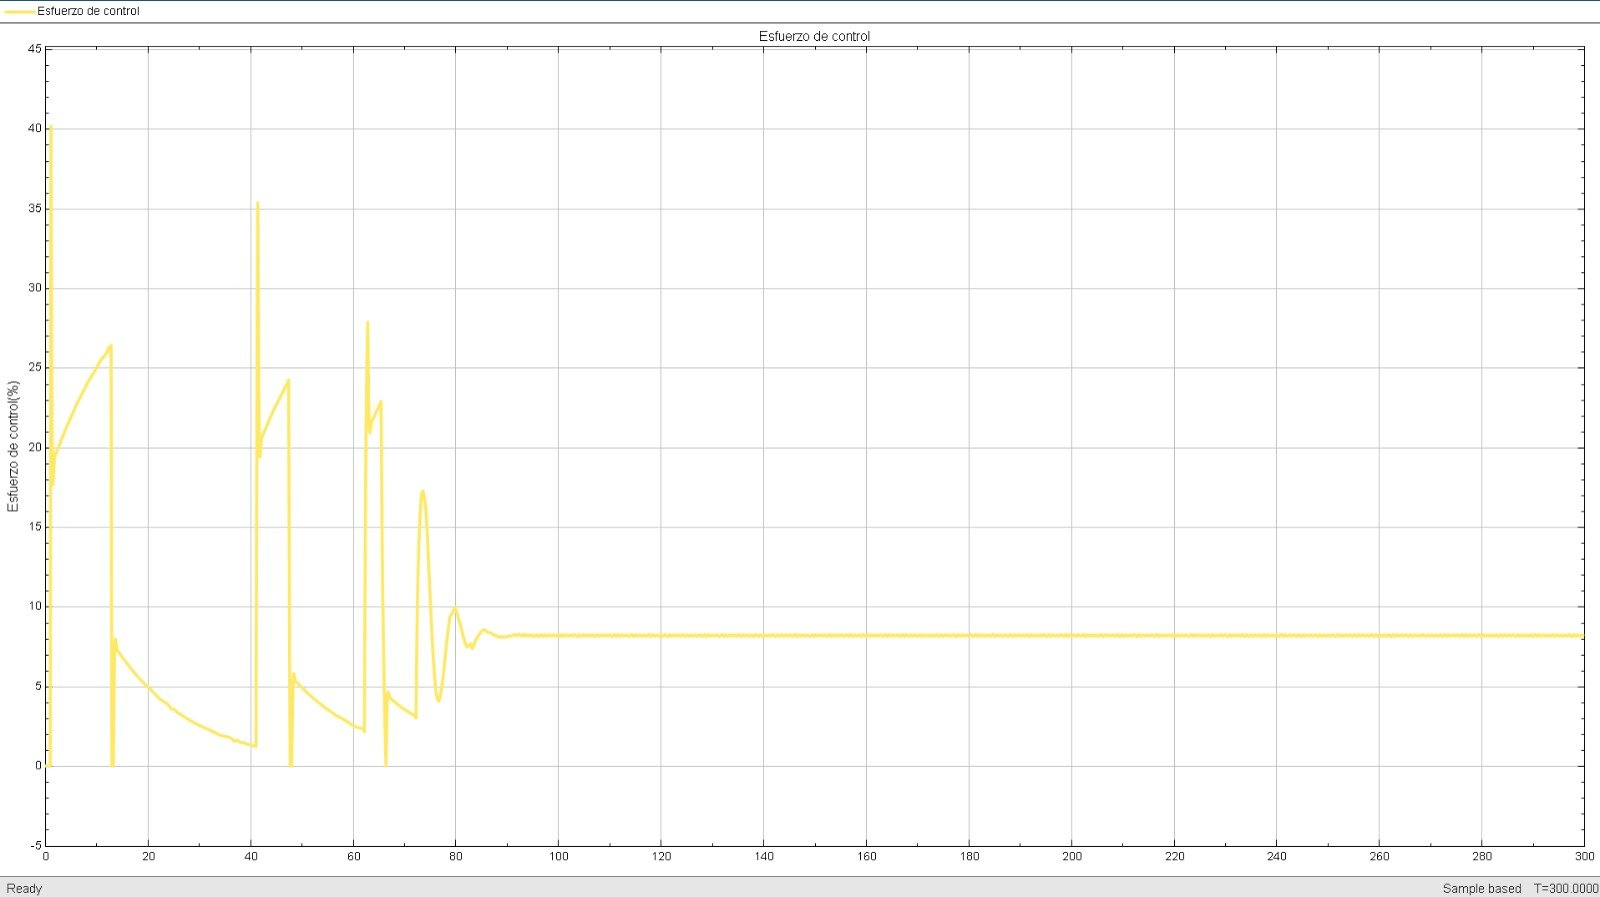
\includegraphics[width=0.95\textwidth]{images/ESFUERZO_FC10.png}
            \caption{Esfuerzo de control de FC10: porcentaje de apertura de EV11.}
            \label{fig:esfuerzo_fc10}
        \end{figure}

        \item Parámetros de desempeño del control de \textbf{FT10}: porcentaje de sobreimpulso, tiempo de establecimiento y error en estado estable.

        Los parámetros del lazo interno FC10, obtenidos del PID Tuner sobre el modelo \(G_{\text{FT10}}(s)\), se presentan en la Tabla~\ref{tab:perf_fc10}. Las tres especificaciones se cumplen con holgura.
        \begin{table}[H]
            \centering
            \begin{tabular}{|l|c|c|}
                \hline
                \textbf{Parámetro} & \textbf{Valor obtenido} & \textbf{Especificación} \\ \hline
                Sobreimpulso \(M_p\) & 6.25\,\% & \(< 10\%\) \\ \hline
                Tiempo de establecimiento \(t_s\) & 1.6 s & \(< 20\) s \\ \hline
                Error en estado estable \(e_{ss}\) & \(\approx 0\,\%\) & \(< 1\%\) \\ \hline
            \end{tabular}
            \caption{Parámetros de desempeño del control de caudal FT10.}
            \label{tab:perf_fc10}
        \end{table}

        \item Parámetros de desempeño del control de nivel \textbf{LC10}: porcentaje de sobreimpulso, tiempo de establecimiento y error en estado estable.

        Los parámetros del lazo externo LC10 se midieron directamente sobre la respuesta simulada del sistema en cascada (Figura~\ref{fig:lc10_nivel}). Se observa un sobreimpulso considerable causado por el \textit{wind-up} del integrador durante la saturación inicial del lazo interno.
        \begin{table}[H]
            \centering
            \begin{tabular}{|l|c|c|}
                \hline
                \textbf{Parámetro} & \textbf{Valor obtenido} & \textbf{Especificación} \\ \hline
                Sobreimpulso \(M_p\) & \(\approx 82\,\%\) (pico 91\,\% sobre SP 50\,\%) & \(< 5\%\) \\ \hline
                Tiempo de establecimiento \(t_s\) & \(\approx 88\,\)s & \(< 200\) s \\ \hline
                Error en estado estable \(e_{ss}\) & \(\approx 0\,\%\) & \(< 5\%\) \\ \hline
            \end{tabular}
            \caption{Parámetros de desempeño del control de nivel LC10.}
            \label{tab:perf_lc10}
        \end{table}

        \textit{Observación:} el sobreimpulso obtenido excede el límite especificado (\(< 5\%\)). Para reducirlo se recomienda habilitar \textit{anti-windup} (back-calculation) en el PID LC10, reducir la ganancia \(K_p\), o re-sintonizar con una respuesta más conservadora. El tiempo de establecimiento y el error en estado estable sí cumplen con sus respectivas especificaciones.
    \end{enumerate}

\end{enumerate}
